\scanpage{5}
\noindent\tikz[baseline=(n.base)]{\node[inner sep=0pt] (n) {D};\draw (n.center) ellipse (.82em and .88em);\draw (n.center) ellipse (1.08em and 1.13em);\draw ([xshift=-1em,yshift=-.35em]n.center) .. controls ([xshift=-1.04em,yshift=.75em]n.center) and ([xshift=-.30em,yshift=1em]n.center) .. ([xshift=.35em,yshift=.96em]n.center);}\quad
\uline{General properties of} \uline{\unsure{abelian|abelian} schemes} \uline{and \unsure{para-abelian|para-abelian}}

\figure{\makebox[\linewidth][l]{\hspace*{3em}\tikz{\foreach \y in {0,.12,.24,.36,.48}{\fill (0,\y) ellipse (.012 and .020);}}}}

\noindent\tikz[baseline=(n.base)]{\node[inner sep=0pt] (n) {E};\draw (n.center) ellipse (.68em and .96em);\draw (n.center) ellipse (.88em and 1.12em);}\quad
\uline{Extensions of \unsure{abelian|abelian} schemes by affine groups}

\noindent\hspace*{7em} (Chevalley's theorem....).

\figure{\makebox[\linewidth][l]{\hspace*{3em}\tikz{\foreach \y/\l in {0/.08,.13/.04,.26/.06,.39/.06,.52/.09}{\draw (0,\y) -- ++(0,\l);}}}}

\noindent%
\figure{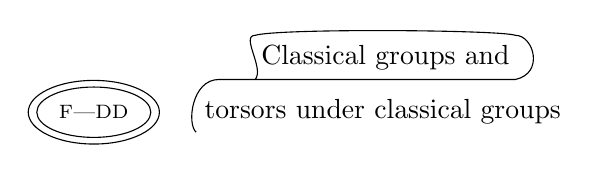
\begin{tikzpicture}[baseline=(t.base)]
\node[anchor=base,font=\scriptsize] (letter) at (-1.40,0) {\deleted{\unsure{F|D}}D};
\draw (letter.center) ellipse (2.06em and .91em);
\draw (letter.center) ellipse (2.37em and 1.15em);
\node[anchor=south west,inner xsep=2pt] (ins) at (.65,.50) {\inserted{Classical groups and}};
\draw (ins.south west) .. controls +(.12,.14) and +(-.19,0) .. (ins.north west)
  .. controls +(.30,.09) and +(-.20,.07) .. (ins.north east)
  .. controls +(.23,0) and +(.37,.08) .. (ins.south east) -- (ins.south west);
\draw (ins.south west) -- (.19,.50) .. controls (-.16,.50) and (-.22,-.07) .. (-.10,-.17);
\node[anchor=base west,inner sep=0pt] (t) at (0,0) {\uline{torsors} \uline{under classical groups}};
\end{tikzpicture}}\margin{(Anywhere)}

\noindent\hfill and theorem of isotriviality over a field \unsure{(P.)|(?)}.

\noindent\tikz[baseline=(n.base)]{\node[inner sep=0pt] (n) {\scriptsize\deleted{\unsure{E|F}}\unsure{F|E}};\draw (n.center) ellipse (2.20em and .95em);\draw (n.center) ellipse (2.40em and 1.18em);}\quad
Néron models (?)

\noindent\hfill A paragraph of variations on the ``theorem \unsure{of the|of the} square''?

\noindent \unsure{References|References}\quad \begin{tabular}[t]{@{}l@{}}
SGAD\\
BIBLE\\
``Boulder''\\
Mumford book(s)
\end{tabular}

% archive sheet number: 4
\clearpage
